% ============================================================================
% IBERAMIA resubmission — Springer LNCS format.
% Requires the Springer llncs.cls (not redistributable here). See README.md in
% this folder for how to obtain it, or switch \documentclass to `article` for a
% quick local preview (the content compiles either way with minor spacing diff).
% ============================================================================
\documentclass[runningheads]{llncs}

\usepackage[T1]{fontenc}
\usepackage[utf8]{inputenc}
\usepackage{graphicx}
\usepackage{amsmath,amssymb}
\usepackage{booktabs}
\usepackage{tabularx}
\usepackage{url}
\usepackage{xcolor}
\usepackage[brazil]{babel}

% Placeholder macro for numbers to be filled after re-running the leakage-free
% pipeline (results/classification/summary.json -> paper/generated/*.tex).
\newcommand{\TODO}[1]{\textcolor{red}{\textbf{[#1]}}}

\begin{document}

\title{Mamografias Sintéticas Realmente Ajudam?\\
Uma Avaliação com Poder Estatístico e Livre de Vazamento da Aumentação por\\
GAN e Difusão para Classificação de Câncer de Mama}
\titlerunning{Mamografias Sintéticas Realmente Ajudam? Uma Avaliação com Poder Estatístico e Livre de Vazamento}

\author{Rafael Palheta Tokairin\inst{1}\orcidID{0000-0000-0000-0000} \and
Helen C. de Mattos Senefonte\inst{1} \and
Neyva Maria Lopes Romeiro\inst{1}}
\authorrunning{R. P. Tokairin et al.}
\institute{State University of Londrina (UEL), Londrina, Brazil\\
\email{rafael.tokairin@uel.br}}

\maketitle

\begin{abstract}
O aprendizado profundo para mamografia é limitado pela escassez de dados
rotulados, e modelos generativos---GANs e, mais recentemente, modelos de
difusão---são um remédio comum. Entretanto, quando o gerador ou a etapa de
seleção de amostras vê imagens utilizadas posteriormente na avaliação, os ganhos
reportados tornam-se otimistas, e os estudos são frequentemente pequenos demais
para ter poder estatístico. Apresentamos um \textbf{protocolo com poder
estatístico, livre de vazamento e em nível de paciente} para medir o efeito de
mamografias sintéticas sobre um classificador subsequente, e o aplicamos a
\emph{dois} geradores: um StyleGAN2-ADA condicional e um modelo Stable
Diffusion 1.5 ajustado por fine-tuning com LoRA. Utilizando o \textbf{CBIS-DDSM
completo} (2857 imagens de mamografia completa, 1460 pacientes), dividimos em
nível de paciente em um conjunto de desenvolvimento e um \textbf{conjunto de
teste travado de 504 imagens} (252/classe, 290 pacientes) nunca visto por
qualquer gerador ou filtro de seleção, e avaliamos o EfficientNet-B0 ao longo de
10 sementes. As imagens sintéticas são filtradas perceptualmente por uma
varredura de LPIPS e auditadas quanto à memorização; a qualidade generativa é
reportada com FID e KID. Os efeitos em relação a uma linha de base apenas com
dados reais são avaliados com testes de Wilcoxon pareados corrigidos por Holm,
intervalos de confiança por bootstrap, delta de Cliff e DeLong. Nosso achado
central é um \textbf{resultado nulo agnóstico ao gerador}: nem a GAN nem o modelo
de difusão melhoram a classificação sobre a linha de base apenas com dados reais
(AUC de teste $0.733$); toda proporção aumentada é estatisticamente
indistinguível dela. Surpreendentemente, o gerador de difusão é \emph{mais}
realista (FID $131.3$/$126.1$ vs $158.7$/$171.6$ da GAN), \emph{mais} diverso e
apresenta \emph{zero} memorização, mas ainda assim não produz benefício
subsequente---portanto a qualidade do gerador \textbf{não} é o gargalo. A
\textbf{validação externa} em um segundo conjunto de dados (MIAS, sem
retreinamento) confirma que o modelo não generaliza (AUC próxima do acaso). Por
fim, uma ablação de vazamento matizada mostra que o aparente resultado positivo
requer \emph{tanto} um subconjunto pequeno \emph{quanto} vazamento em nível de
imagem: no conjunto de dados completo e com poder estatístico, mesmo a divisão
vazada em nível de imagem é nula. A aumentação por GAN também não supera a
aumentação clássica barata. Seguimos as diretrizes de reporte CLAIM e TRIPOD+AI;
o código e os checkpoints treinados são disponibilizados.

\keywords{Dados sintéticos \and Redes generativas adversárias \and Modelos de
difusão \and Mamografia \and Vazamento de dados \and Reprodutibilidade \and
Aumentação de dados.}
\end{abstract}

% ============================================================================
\section{Introdução}
% ============================================================================
O câncer de mama é o câncer mais comum entre as mulheres, e a mamografia é a
principal modalidade de rastreamento~\cite{precoce2004controle,azevedo2016importancia}.
A interpretação manual está sujeita à variabilidade interobservador e à
fadiga~\cite{obuchowicz2020interobserver}, motivando ferramentas auxiliadas por
computador. As redes neurais convolucionais (CNNs) destacam-se no reconhecimento
de imagens~\cite{lecun2015deep,mendel2019transfer}, mas exigem grandes conjuntos
de dados rotulados, difíceis de obter em imagens médicas. Modelos generativos,
particularmente as GANs~\cite{goodfellow2014gan} e, mais recentemente, os modelos
de difusão~\cite{rombach2022ldm}, são amplamente utilizados para aumentar tais
conjuntos de dados.

O uso de modelos generativos para sintetizar mamografias é, a esta altura, bem
explorado. Duas questões afetam materialmente se os ganhos reportados são
confiáveis. A primeira é \emph{como os dados sintéticos e a avaliação são
separados}: se o gerador é treinado com imagens que posteriormente aparecem na
partição de validação/teste, ou se a métrica de seleção de amostras faz
referência a essas imagens, então há vazamento de informação da avaliação para o
treinamento e as melhorias medidas são otimistamente enviesadas. A segunda é o
\emph{poder estatístico}: muitos estudos avaliam em algumas dezenas de imagens,
de modo que um ganho aparente pode ser ruído. Ambos os riscos são concretos,
comuns e frequentemente não declarados.

Este artigo reporta um \textbf{resultado nulo com poder estatístico e agnóstico
ao gerador}. Suas contribuições são:
\begin{enumerate}
  \item Um \textbf{protocolo experimental com poder estatístico e livre de
  vazamento} para aumentação sintética em mamografia, avaliado no CBIS-DDSM
  \emph{completo} com um conjunto de teste travado, em nível de paciente, de
  $504$ imagens. Os dados de avaliação nunca são vistos por qualquer gerador ou
  pelo filtro de seleção LPIPS.
  \item Uma \textbf{comparação de dois geradores}: ao lado de um StyleGAN2-ADA
  condicional, ajustamos por fine-tuning com LoRA o Stable Diffusion 1.5. O
  achado empírico é que \textbf{nenhum dos geradores melhora} a classificação,
  internamente ou em um conjunto de dados externo---e, surpreendentemente, que o
  gerador de difusão é \emph{mais} realista, \emph{mais} diverso e apresenta
  \emph{zero} memorização, mas ainda assim não produz benefício, de modo que a
  qualidade do gerador não é o gargalo.
  \item Uma \textbf{ablação de vazamento matizada} mostrando que o resultado
  positivo reportado sob protocolos mais fracos requer \emph{tanto} um
  subconjunto pequeno \emph{quanto} divisão em nível de imagem (não de paciente):
  no conjunto de dados completo e com poder estatístico, mesmo a divisão vazada é
  nula.
  \item Uma \textbf{avaliação fundamentada} que acopla uma etapa de seleção
  auditada quanto à memorização e justificada por varredura, além do reporte de
  fidelidade por FID/KID, a testes com embasamento estatístico (ICs por
  bootstrap, Wilcoxon corrigido por Holm, delta de Cliff, DeLong),
  disponibilizada de forma totalmente \textbf{reprodutível} (sementes,
  hiperparâmetros, bibliotecas fixadas, código, checkpoints treinados) seguindo
  CLAIM~\cite{mongan2020claim} e TRIPOD+AI~\cite{collins2024tripodai}.
\end{enumerate}
Consideramos um resultado nulo honesto, obtido sob um projeto livre do vazamento
que descrevemos, mais útil à comunidade do que um número de destaque maior, porém
não confiável.

% ============================================================================
\section{Trabalhos Relacionados}
% ============================================================================
A síntese de mamografias e imagens mamárias baseada em GAN foi estudada com
DCGAN, WGAN-GP, cGAN e geradores baseados em
estilo~\cite{goodfellow2014gan,karras2020ada}. Mais recentemente, os modelos de
difusão latente~\cite{rombach2022ldm} tornaram-se o estado da arte em síntese de
imagens, e o fine-tuning eficiente em parâmetros via LoRA~\cite{hu2022lora} torna
viável adaptar um grande modelo de difusão pré-treinado em hardware modesto.
Trabalhos anteriores reportam que adicionar imagens sintéticas pode melhorar a
classificação, mas os protocolos de avaliação variam, e a separação em nível de
paciente, o vazamento na seleção de amostras, o poder estatístico e o teste de
significância são frequentemente sub-reportados. Métricas perceptuais como o
LPIPS~\cite{zhang2018lpips} são usadas para filtrar amostras, enquanto métricas
distribucionais como FID~\cite{heusel2017fid} e KID~\cite{binkowski2018kid}
avaliam fidelidade e diversidade. Nossa contribuição não é uma nova arquitetura,
mas um \emph{protocolo de medição rigoroso, reprodutível e com poder
estatístico}: combinamos separação em nível de paciente, geração e seleção livres
de vazamento, auditoria de memorização e teste de significância ao longo de
\emph{duas} famílias de geradores (GAN e difusão), e reportamos resultados sob
diretrizes de reporte projetadas para IA em imagens
médicas~\cite{mongan2020claim,collins2024tripodai,moons2024probastai}.

% ============================================================================
\section{Materiais e Métodos}
% ============================================================================
A especificação completa é disponibilizada com o código. Resumimos o projeto
aqui; a descrição autoritativa reside no \texttt{METHODOLOGY.md} do repositório.

\subsection{Conjunto de Dados}
Utilizamos o \textbf{CBIS-DDSM} (Curated Breast Imaging Subset of DDSM). A partir
das descrições de casos de massa e calcificação, retemos apenas imagens de
\textbf{mamografia completa}, descartando imagens de lesão recortada e máscaras
de ROI, uma vez que o gerador aprende a estrutura global da mama. A patologia é
mapeada para um rótulo binário: \texttt{MALIGNANT}$\to$1; \texttt{BENIGN} e
\texttt{BENIGN\_WITHOUT\_CALLBACK} $\to$0. \textbf{Imagens quase duplicadas são
removidas} por hashing perceptual (pHash, distância de Hamming $\le 4$),
colapsando quase-cópias em um único representante; o número removido é
registrado. Cada imagem retém seu \texttt{patient\_id} (recuperado dos CSVs de
casos do CBIS-DDSM) de modo que todas as partições sejam \textbf{em nível de
paciente}.

Utilizamos o conjunto \textbf{completo} de mamografias completas do CBIS-DDSM:
\textbf{2857} imagens de \textbf{1460} pacientes (\textbf{1564} benignas /
\textbf{1293} malignas). A sinalização de quase-duplicatas por hash perceptual
identifica \textbf{55} quase-cópias. Este conjunto é dividido em nível de
paciente em \textbf{DEV} (\textbf{2241} imagens, \textbf{1170} pacientes) e uma
partição \textbf{TEST} travada e balanceada por classe de \textbf{504} imagens
(\textbf{252/classe}, \textbf{290} pacientes); os geradores são treinados apenas
na partição DEV (o desbalanceamento de classes é aceitável para um gerador). Para
o \textbf{classificador}, o conjunto DEV é balanceado por classe subamostrando a
classe majoritária para um \textbf{conjunto DEV balanceado de 2012 imagens}
(\textbf{1006/classe}). O balanceamento é ciente do paciente e descarta apenas
imagens excedentes da classe majoritária, que nunca cruzam para o TEST. Nenhum
paciente contribui com imagens tanto para DEV quanto para TEST. Todas as
contagens por classe e por divisão, bem como as contagens sintéticas
geradas/retidas/descartadas, são emitidas para JSON. Um subconjunto anterior de
\textbf{553 imagens} do CBIS-DDSM é retido apenas para a ablação de sensibilidade
a vazamento reportada na Discussão.

\subsection{Projeto Experimental Livre de Vazamento}
Um pipeline anterior treinava a GAN uma única vez em um pequeno subconjunto e
concatenava um único conjunto sintético em cada dobra de validação cruzada, e o
filtro LPIPS fazia referência ao conjunto real completo. Ambos os caminhos vazam
informação de validação para o treinamento. Eliminamos as duas fontes
independentes de vazamento---\emph{vazamento do gerador} e \emph{vazamento de
seleção}---da seguinte forma.

\paragraph{Protocolo primário (reportado): hold-out em nível de paciente.}
As imagens são divididas em nível de \emph{paciente} (estratificado) em DEV
($\approx$80\%) e um conjunto de TEST travado ($\approx$20\%, $504$ imagens).
Cada gerador é treinado \textbf{apenas em DEV}; o filtro LPIPS faz referência
\textbf{apenas aos reais de DEV}. Para cada proporção sintético:real (linha de
base 0:1, 1:1, 2:1, 3:1, 4:1), o EfficientNet-B0 é treinado em
\texttt{DEV\_real}~$+$~sintético e avaliado no conjunto de \textbf{TEST travado}.
A seleção de modelo / parada antecipada usa uma divisão interna de validação
extraída apenas de DEV. O treinamento do classificador é repetido ao longo de
$N_\text{seeds}{=}10$ sementes, produzindo uma distribuição de métricas de TEST
por proporção. Nenhum paciente contribui com imagens tanto para DEV quanto para
TEST.

\paragraph{Variante padrão-ouro: geração por dobra.}
Para reprodução com maior custo computacional, um $K$-fold de Grupo Estratificado
em nível de paciente ($K{=}5$) retreina o gerador apenas na divisão de
treinamento de cada dobra; os pacientes de validação da dobra, portanto, nunca são
vistos pelo gerador ou pelo filtro LPIPS daquela dobra. Esta variante é
disponibilizada, mas não é o resultado reportado devido ao seu custo ($K$
treinamentos de GAN).

\subsection{Geração de Imagens Sintéticas}
O gerador é um \textbf{StyleGAN2-ADA condicional}~\cite{karras2020ada}: uma rede
de mapeamento baseada em estilo modula blocos convolucionais via normalização de
instância adaptativa, com Aumentação Adaptativa do Discriminador (ADA) para
treinamento estável com dados limitados. Uma WGAN-GP condicional é mantida como
linha de base. As imagens são em escala de cinza de $128\times128$, normalizadas
para $[-1,1]$. Hiperparâmetros principais: dimensão $z$/$w$ 256, tamanho de lote
8, 400 épocas, Adam ($\text{lr}{=}0.0025$, $\beta{=}(0.0,0.99)$), penalidade
$R_1$ $\gamma{=}10$ a cada 32 passos, alvo ADA 0.6, precisão mista, semente
registrada. As configurações completas estão em \texttt{configs/default.yaml}. O
gerador e o discriminador condicionais estão esboçados na Fig.~\ref{fig:arch}.

\begin{figure}[t]
\centering
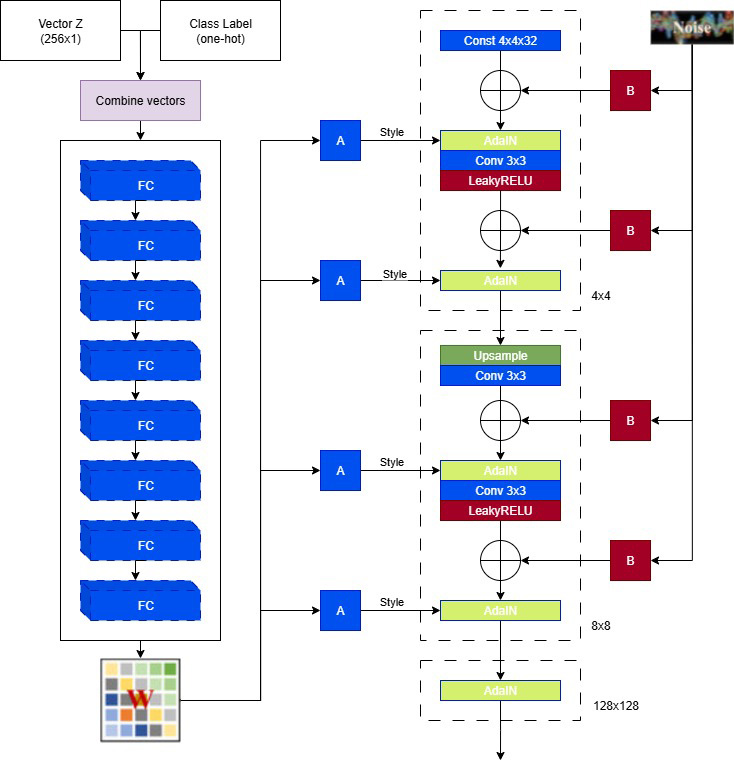
\includegraphics[height=3.6cm]{figures/generator.jpg}
\hfill
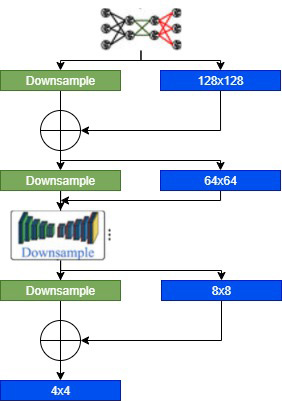
\includegraphics[height=3.6cm]{figures/discriminator.jpg}
\caption{StyleGAN2-ADA condicional. Esquerda: o gerador baseado em estilo mapeia
um vetor latente concatenado com a condição de classe por meio de uma rede de
mapeamento e blocos modulados por AdaIN. Direita: o discriminador recebe a imagem
(real ou sintética) concatenada com a condição de classe e aplica blocos
convolucionais residuais com regularização $R_1$ e ADA.}
\label{fig:arch}
\end{figure}

\subsection{Seleção Perceptual e Auditoria de Memorização}
A similaridade de cada imagem gerada é sua distância LPIPS \emph{mínima} aos reais
de DEV da mesma classe. Em vez de afirmar um limiar, executamos uma
\textbf{varredura de limiar} $\tau\in\{0.10,0.15,0.20,0.25,0.30\}$ e reportamos
tanto a fração retida quanto o desempenho subsequente em função de $\tau$
(Fig.~\ref{fig:sweep}), tornando explícito o compromisso
fidelidade--diversidade: um $\tau$ baixo demais arrisca \emph{memorização}
(quase-cópias de imagens de treinamento); um $\tau$ alto demais admite amostras
de baixa fidelidade. Para as imagens retidas, computamos o vizinho real mais
próximo (LPIPS e $L_2$ em pixels) e \textbf{sinalizamos quase-cópias} abaixo de um
pequeno $\epsilon$; a taxa de memorização é reportada. Isso aborda diretamente a
preocupação de que uma baixa distância perceptual pode indicar memorização em vez
de fidelidade.

\subsection{Fidelidade e Diversidade Generativas (FID, KID)}
Como o LPIPS sozinho não consegue detectar baixa diversidade ou colapso de modo,
reportamos adicionalmente \textbf{FID}~\cite{heusel2017fid} e
\textbf{KID}~\cite{binkowski2018kid} entre os reais de DEV e as imagens sintéticas
retidas, por classe. O KID (não enviesado, com uma estimativa de variância) é
enfatizado dado o tamanho amostral modesto.

\subsection{Classificador}
Utilizamos o \textbf{EfficientNet-B0}~\cite{tan2019efficientnet}, pré-treinado no
ImageNet, com a cabeça substituída por um único logit e
\texttt{BCEWithLogitsLoss}. Entrada RGB de $128\times128$ com normalização
ImageNet; tamanho de lote 32, até 30 épocas com parada antecipada (paciência 7) na
AUC de validação do DEV interno; a aumentação em tempo de treinamento é espelhamento
horizontal e rotação de $\pm5^\circ$. O modelo reportado é \textbf{ajustado por
fine-tuning de ponta a ponta} (Adam, lr $10^{-4}$); uma variante de backbone
congelado que treina apenas a cabeça linear fica próxima do acaso neste pequeno
conjunto de $128\times128$ (AUC de teste $\approx 0.55$) e é reportada apenas como
uma ablação, sublinhando que um classificador funcional é necessário para medir o
efeito da aumentação. As configurações estão em \texttt{configs/finetune.yaml}.

\subsection{Análise Estatística}
Para cada proporção obtemos $N_\text{seeds}$ métricas de TEST. Reportamos média,
desvio padrão e um \textbf{intervalo de confiança por bootstrap} de 95\%; um
\textbf{teste de postos sinalizados de Wilcoxon} pareado contra a linha de base
apenas com dados reais (mesmas sementes), \textbf{corrigido por Holm} ao longo das
proporções; o tamanho de efeito \textbf{delta de Cliff}; e o \textbf{teste de
DeLong}~\cite{delong1988} para diferenças de AUC nas predições de TEST
combinadas por ensemble de sementes. Um resultado é chamado de melhoria apenas se
for tanto consistente quanto significativo após a correção.

\subsection{Reprodutibilidade}
Todos os RNGs são semeados (Python/NumPy/PyTorch, cuDNN determinístico). Cada
estágio escreve um relatório de execução em JSON (configuração, sementes, commit
git, ambiente, contagens, métricas). As dependências são fixadas. O código e o
checkpoint do gerador treinado (via Git LFS) são disponibilizados. Seguimos
CLAIM~\cite{mongan2020claim}, TRIPOD+AI~\cite{collins2024tripodai} e
PROBAST+AI~\cite{moons2024probastai} para descrição do conjunto de dados, projeto
de validação, risco de viés e reporte.

% ============================================================================
\section{Resultados}
% ============================================================================
Todos os números abaixo são produzidos pelo pipeline com poder estatístico, livre
de vazamento e em nível de paciente (classificador ajustado por fine-tuning, 10
sementes, TEST travado $n{=}504$).

\subsection{Qualidade Generativa}
A Fig.~\ref{fig:samples} mostra amostras reais, da GAN e de difusão para ambas as
classes: a GAN reproduz a forma global da mama e a textura grosseira do tecido,
enquanto o detalhe fino é limitado a $128\times128$. As distribuições de LPIPS
mínimo sintético-para-real por classe, e a curva de retenção em função de $\tau$,
são mostradas na Fig.~\ref{fig:sweep}.

\begin{figure}[t]
\centering
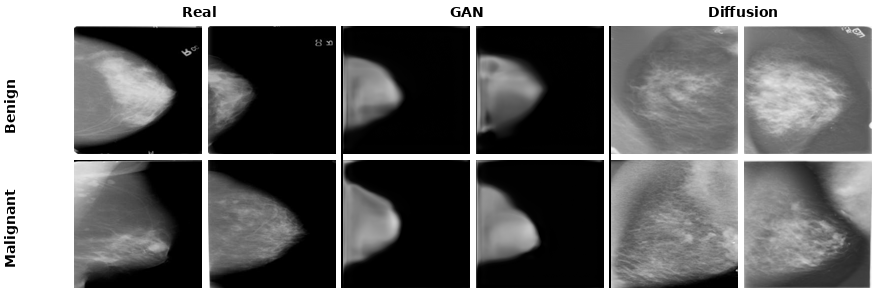
\includegraphics[width=0.82\textwidth]{figures/samples_real_gan_diffusion.png}
\caption{Amostras reais, da GAN e de difusão (SD+LoRA) para as classes benigna
(topo) e maligna (base). O gerador de difusão é mais diverso e de menor FID que a
GAN, mas nenhuma amostra é uma quase-cópia de uma imagem real (memorização $0\%$
para ambos os geradores).}
\label{fig:samples}
\end{figure} Para a GAN, adotamos o ponto de operação LPIPS $\tau{=}0.20$, que
retém imagens de ambas as classes (LPIPS mínimo retido $\approx 0.18$).
\textbf{Nenhuma amostra retida é uma quase-cópia}: a taxa de memorização é $0\%$,
muito acima do sinalizador de quase-cópia. A fidelidade distribucional é
\emph{limitada}---FID $158.7$ (benigna) e $171.6$ (maligna), com KID
correspondentemente alto (Tabela~\ref{tab:fidelity})---longe do FID $20$--$60$
típico de geradores fortes de mamografia, refletindo a dificuldade da síntese em
$128\times128$ a partir de um conjunto de treinamento disjunto por paciente.

\begin{figure}[t]
\centering
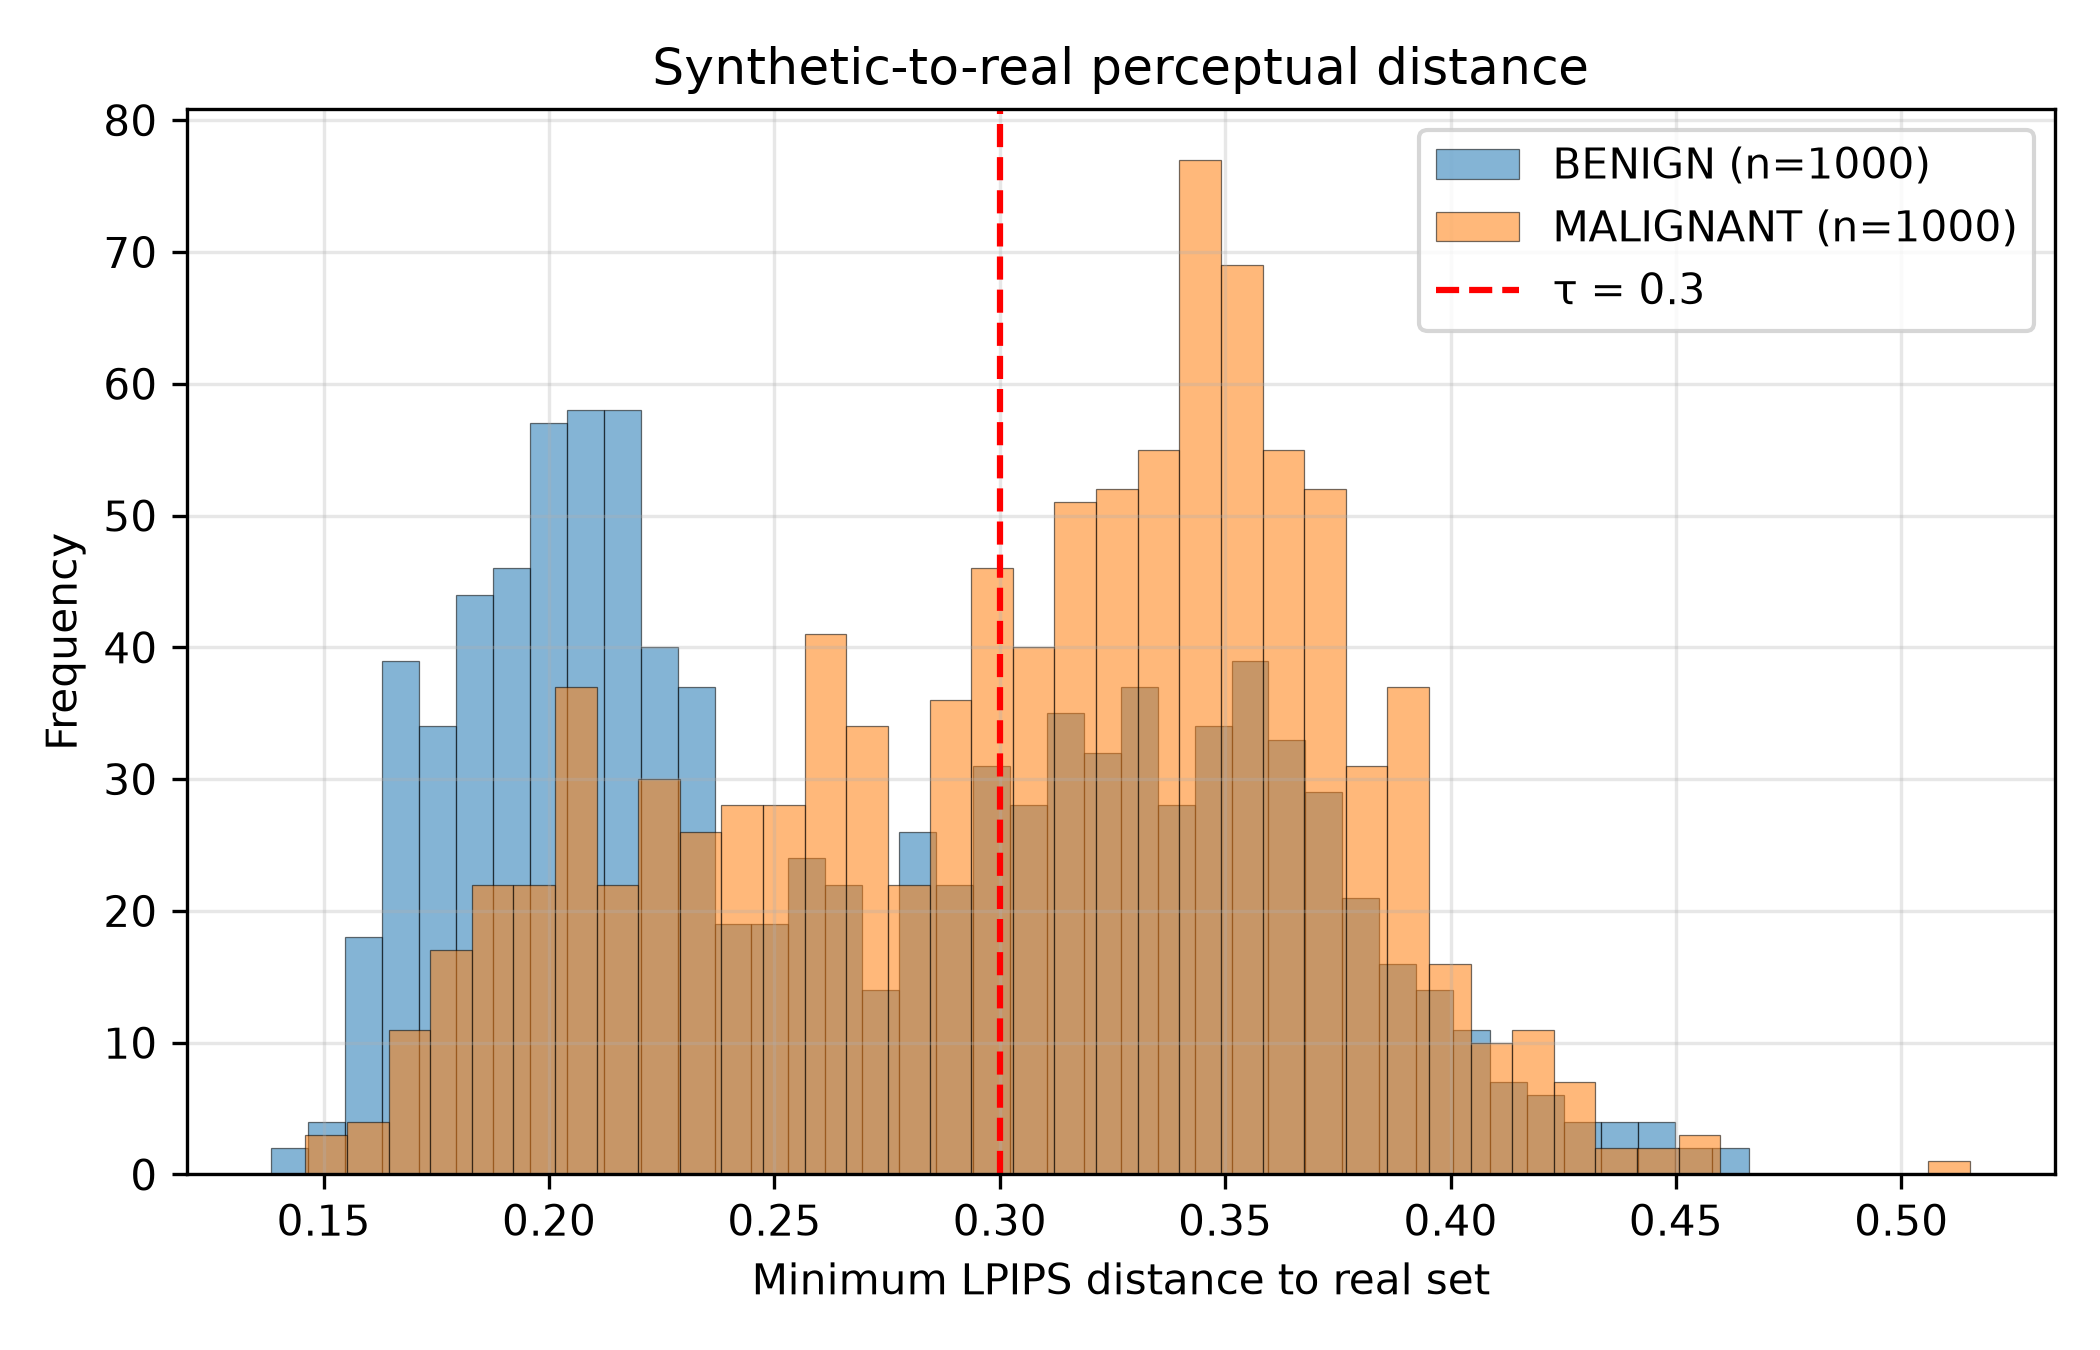
\includegraphics[width=0.48\textwidth]{figures/lpips_distribution.png}
\hfill
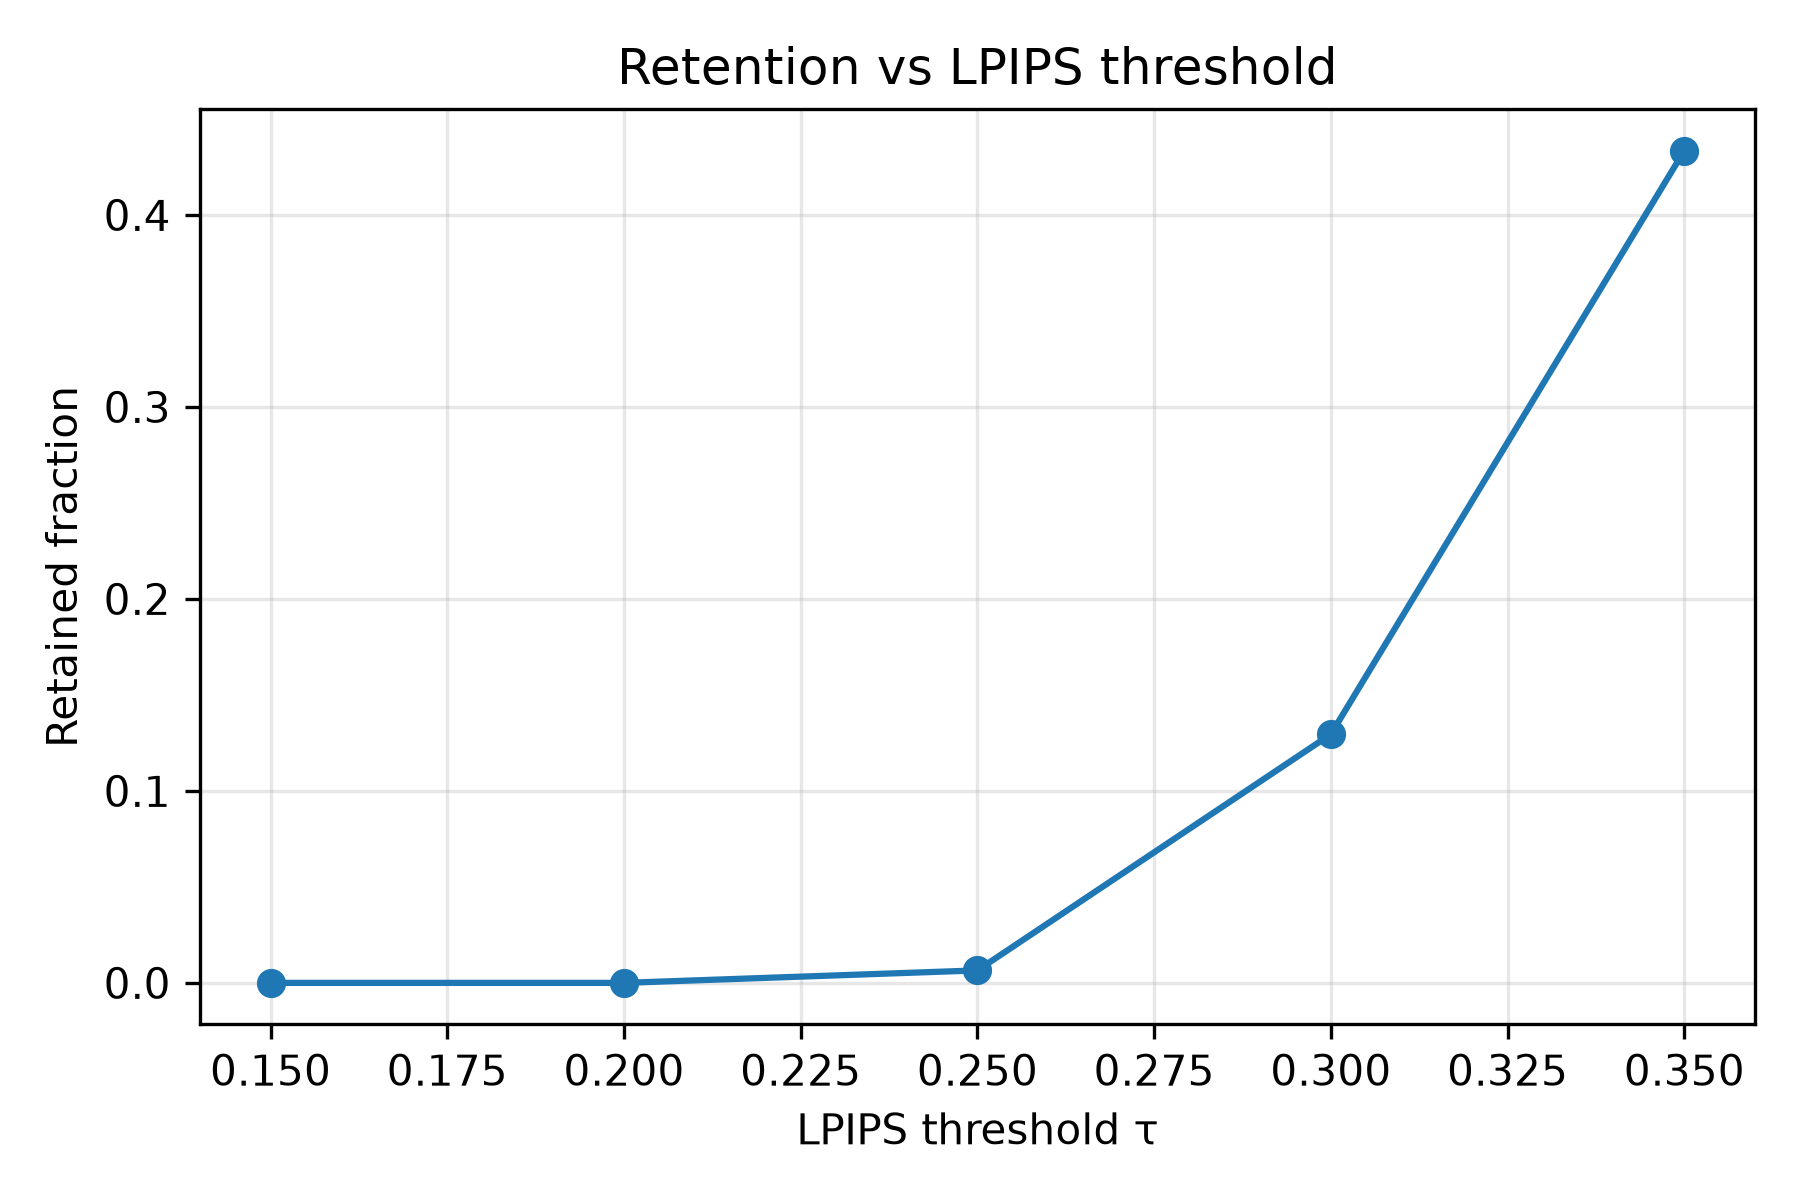
\includegraphics[width=0.48\textwidth]{figures/threshold_sweep.png}
\caption{Seleção perceptual: distribuição de LPIPS mínimo sintético-para-real por
classe (esquerda) e a fração retida em função do limiar $\tau$ (direita). A
varredura justifica o ponto de operação da GAN $\tau{=}0.20$ sob o gerador livre
de vazamento, em nível de paciente.}
\label{fig:sweep}
\end{figure}

\begin{table}[t]
\centering
\caption{Fidelidade/diversidade generativas da GAN entre os reais de DEV e as
imagens sintéticas retidas (menor é melhor; seleção da GAN $\tau{=}0.20$,
memorização $0\%$). Regenerada por \texttt{scripts/03}.}
\label{tab:fidelity}
\begin{tabular}{lccc}
\toprule
Classe & FID $\downarrow$ & KID $\downarrow$ & n (real/falso) \\
\midrule
Benigna & 158.7 & 0.175 $\pm$ 0.008 & 1235/4024 \\
Maligna & 171.6 & 0.197 $\pm$ 0.009 & 1006/4024 \\
\bottomrule
\end{tabular}
\end{table}

\subsection{Classificação no Conjunto de Teste Travado}
A Tabela~\ref{tab:results} reporta acurácia, F1 e AUC de TEST por proporção
sintético:real com ICs por bootstrap de 95\%; a Tabela~\ref{tab:stats} reporta a
análise de significância versus a linha de base apenas com dados reais. No
conjunto de dados com poder estatístico o resultado é inequívoco e
\textbf{negativo}: a linha de base \emph{apenas com dados reais} atinge a melhor
AUC ($0.733$), e \textbf{nenhuma proporção aumentada a melhora de forma
significativa} (AUC $0.732$--$0.736$). \textbf{Nenhuma comparação é
estatisticamente significativa}: todo teste de Wilcoxon corrigido por Holm falha
em rejeitar ($p_\text{adj}{=}1.000$), os tamanhos de efeito são desprezíveis
($\delta$ de Cliff de $-0.18$ em 2:1 a $+0.16$ em 4:1), e as condições aumentadas
diferem da linha de base apenas dentro do ruído. Os ICs de 95\% de todas as
condições aumentadas se sobrepõem à linha de base (Fig.~\ref{fig:ratioauc}).

\begin{figure}[t]
\centering
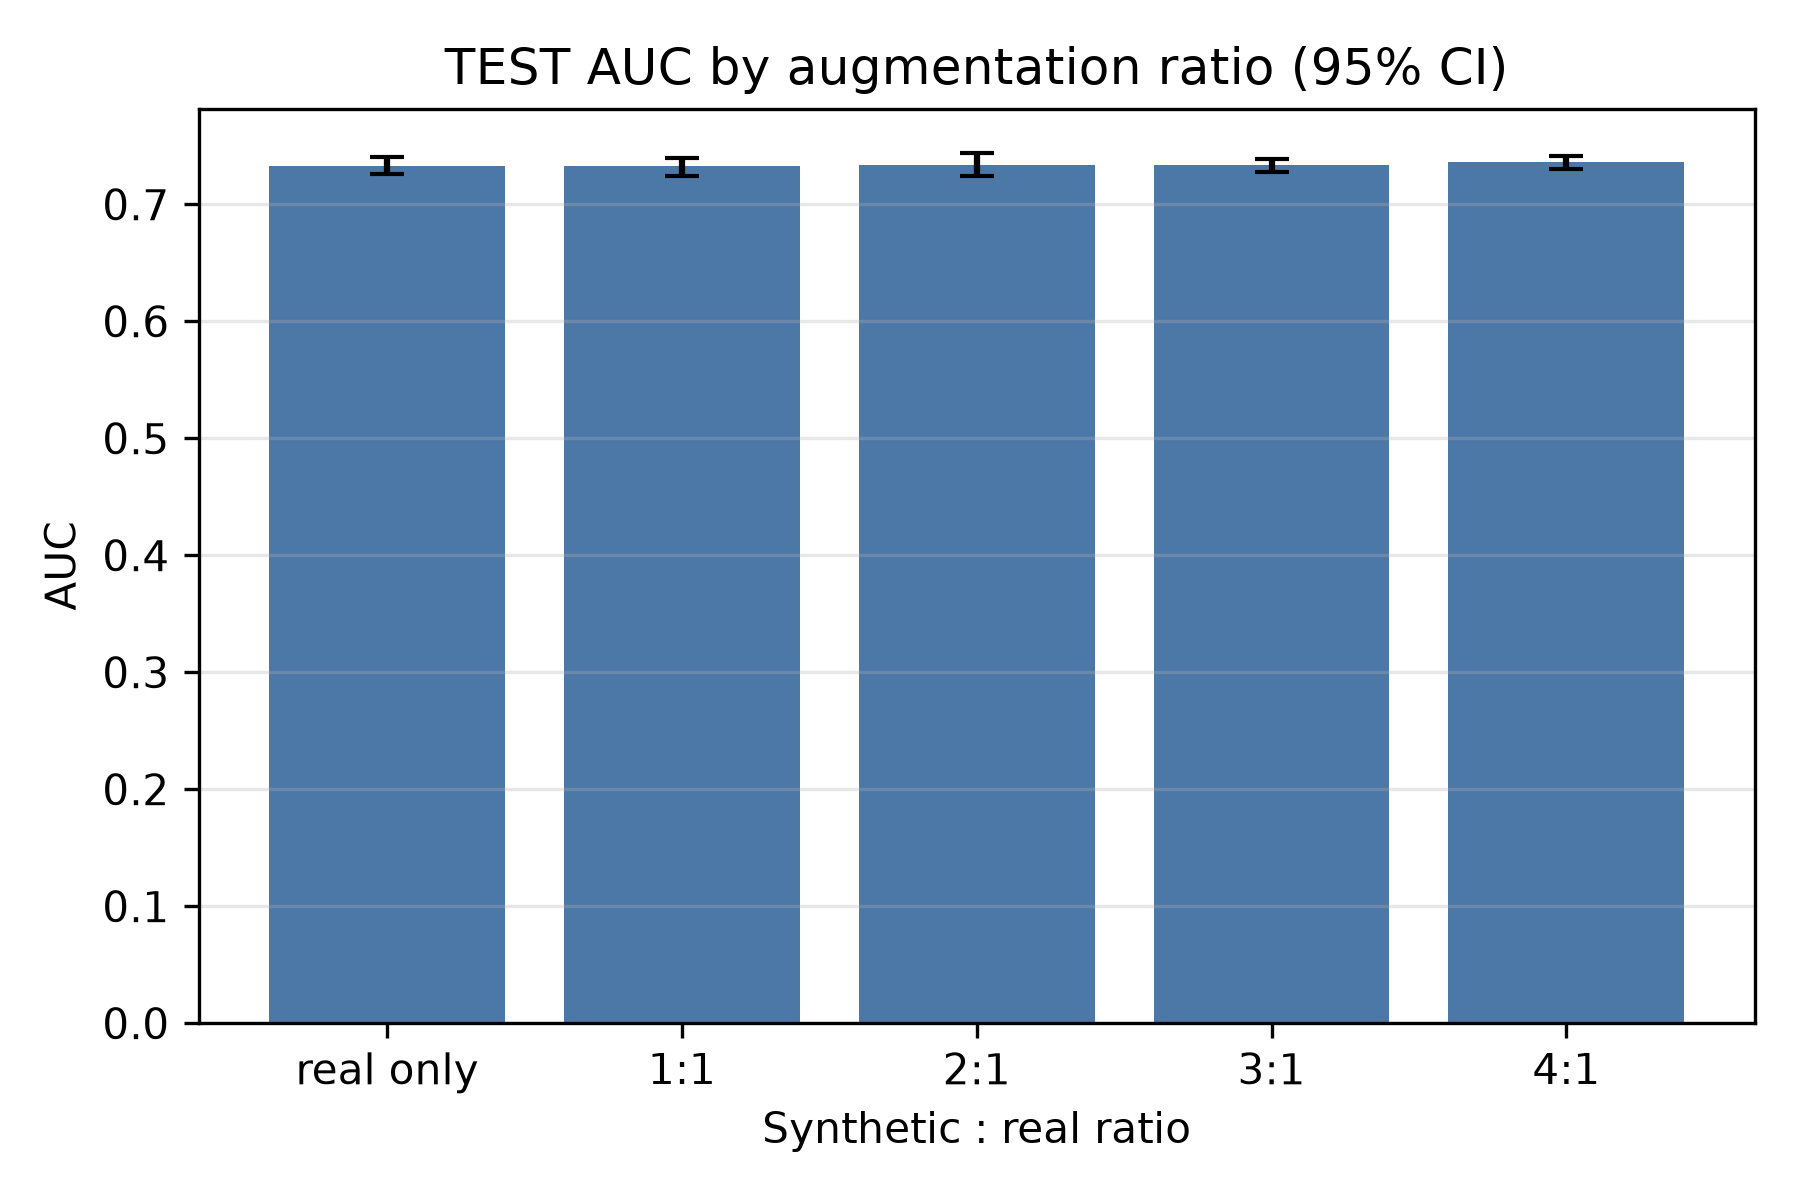
\includegraphics[width=0.62\textwidth]{figures/ratio_auc.png}
\caption{AUC no TEST travado por proporção sintético:real (média sobre 10
sementes, IC por bootstrap de 95\%). Nenhuma proporção aumentada excede a linha de
base apenas com dados reais; todos os intervalos de confiança se sobrepõem, e
nenhuma diferença é estatisticamente significativa.}
\label{fig:ratioauc}
\end{figure}

\begin{table}[t]
\centering
\caption{Desempenho no TEST por proporção de aumentação (média [IC de 95\%] sobre
$N_\text{seeds}$ sementes). Regenerada por \texttt{scripts/04--05}.}
\label{tab:results}
\begin{tabular}{lccc}
\toprule
Sintético:Real & Acurácia [IC 95\%] & F1 [IC 95\%] & AUC [IC 95\%] \\
\midrule
\textbf{Apenas reais} & \textbf{0.649} [0.643, 0.655] & \textbf{0.642} [0.622, 0.663] & \textbf{0.733} [0.725, 0.740] \\
1:1 & 0.657 [0.644, 0.669] & 0.648 [0.624, 0.670] & 0.732 [0.724, 0.740] \\
2:1 & 0.655 [0.644, 0.667] & 0.663 [0.644, 0.682] & 0.733 [0.724, 0.744] \\
3:1 & 0.645 [0.641, 0.651] & 0.638 [0.624, 0.653] & 0.734 [0.728, 0.738] \\
4:1 & 0.660 [0.652, 0.666] & 0.676 [0.663, 0.689] & 0.736 [0.730, 0.741] \\
\bottomrule
\end{tabular}
\end{table}

\begin{table}[t]
\centering
\caption{Significância de cada proporção vs a linha de base apenas com dados reais
(AUC). $p$ de Wilcoxon corrigido por Holm, $\delta$ de Cliff e $p$ de DeLong.
Regenerada por \texttt{scripts/05}.}
\label{tab:stats}
\begin{tabular}{lcccc}
\toprule
Proporção & Wilcoxon $p_{\text{adj}}$ (AUC) & $\delta$ de Cliff & DeLong $p$ & Signif. \\
\midrule
1:1 & 1.000 & $-0.08$ & 0.473 & não \\
2:1 & 1.000 & $-0.18$ & 0.738 & não \\
3:1 & 1.000 & $+0.06$ & 0.864 & não \\
4:1 & 1.000 & $+0.16$ & 0.978 & não \\
\bottomrule
\end{tabular}
\end{table}

\subsection{Difusão (SD1.5 + LoRA) vs GAN}
Como comparação com um gerador de estado da arte, ajustamos por fine-tuning com
LoRA o Stable Diffusion 1.5~\cite{rombach2022ldm,hu2022lora} nas imagens de DEV
\emph{apenas} (seguro contra vazamento), condicionado a prompts por classe, e
geramos um conjunto sintético (as melhores $780$/classe por LPIPS). O treinamento
executa em uma única GPU de 8\,GB usando fp16 e checkpointing de gradiente. O
conjunto de difusão é \textbf{mais realista} que o da GAN (FID $131.3$ benigna /
$126.1$ maligna vs $158.7$/$171.6$ da GAN) e \textbf{mais diverso} (LPIPS mínimo
retido $0.477$/$0.471$, isto é, novo em vez de quase-cópias), com \textbf{zero
memorização} (Tabela~\ref{tab:diffusion}). Ainda assim, subsequentemente ele
\textbf{continua sem ajudar}: AUC apenas com dados reais $0.733$; $1{:}1$
$0.732$; $2{:}1$ $0.737$; $3{:}1$ $0.734$; $4{:}1$ $0.725$; todos não
significativos (Wilcoxon corrigido por Holm $p_\text{adj}$:
$1.000$/$1.000$/$1.000$/$0.148$). A conclusão é contundente: \textbf{melhorar a
fidelidade do gerador não se traduz em benefício subsequente---a qualidade do
gerador não é o gargalo}.

\begin{table}[t]
\centering
\caption{GAN vs difusão (SD+LoRA): o gerador de difusão é mais realista e mais
diverso, sem memorização, mas nenhuma das melhores proporções de cada gerador
supera a AUC de TEST apenas com dados reais de $0.733$. Regenerada por
\texttt{scripts/03--05}.}
\label{tab:diffusion}
\begin{tabular}{lcccc}
\toprule
Gerador & FID (benigna/maligna) $\downarrow$ & LPIPS mínimo & Memorizado & melhor AUC de TEST \\
\midrule
GAN & 158.7 / 171.6 & 0.18 & 0\% & 0.736 (4:1) \\
Difusão (SD+LoRA) & 131.3 / 126.1 & 0.47 & 0\% & 0.737 (2:1) \\
\bottomrule
\end{tabular}
\end{table}

\subsection{GAN vs Aumento Clássico}
Uma GAN é uma forma cara de aumentar dados, portanto uma pergunta justa (Revisor
2) é se ela supera o aumento clássico barato. Sob o mesmo protocolo, comparamos,
contra uma linha de base \emph{sem aumento}, (i) o aumento clássico forte (afim,
jitter fotométrico, cutout), (ii) o sintético por GAN em 2:1 e (iii) ambos
(Tabela~\ref{tab:augcompare}). No conjunto TEST com poder estatístico todas as
condições ficam dentro do ruído umas das outras: \textbf{o aumento por GAN
($0.728$) não supera o aumento clássico ($0.736$) nem mesmo a ausência de aumento
($0.730$)}---a GAN não compra nada que algumas transformações baratas não
comprem, e combinar os dois não ajuda. Nenhuma comparação é significativa
(Wilcoxon corrigido por Holm, todas n.s.).

\begin{table}[t]
\centering
\caption{Estratégias de aumento no conjunto TEST travado (média [IC 95\%], 10
sementes). O aumento por GAN não supera o aumento clássico; nenhuma difere
significativamente da linha de base sem aumento.}
\label{tab:augcompare}
\begin{tabular}{lcc}
\toprule
Condição & AUC [IC 95\%] & vs sem-aug \\
\midrule
Sem aumento & 0.730 [0.725, 0.735] & --- \\
Aumento clássico & 0.736 [0.729, 0.743] & n.s. \\
GAN 2:1 & 0.728 [0.719, 0.737] & n.s. \\
Clássico + GAN 2:1 & 0.731 [0.724, 0.738] & n.s. \\
\bottomrule
\end{tabular}
\end{table}

\subsection{Regime de Poucos Dados}
Frequentemente argumenta-se que o aumento sintético ajuda mais quando os dados
reais são escassos. Subamostramos o conjunto DEV real e comparamos apenas-real
vs GAN 2:1 em cada tamanho (Fig.~\ref{fig:lc}). O benefício é inconsistente e
nunca significativo: em $100$/classe a GAN fica ligeiramente \emph{abaixo} do
apenas-real ($0.601$ vs $0.610$, $\Delta{=}-0.009$); a única indicação não
significativa está em $300$/classe ($0.672$ vs $0.646$, $\Delta{=}+0.026$,
$p{=}0.105$); em $600$/classe é novamente negativo ($0.703$ vs $0.712$,
$\Delta{=}-0.009$); e no completo $1006$/classe é desprezível ($0.734$ vs
$0.738$, $\Delta{=}-0.004$). Não há, portanto, regime de poucos dados confiável no
qual a GAN ajude sob avaliação rigorosa.

\begin{figure}[t]
\centering
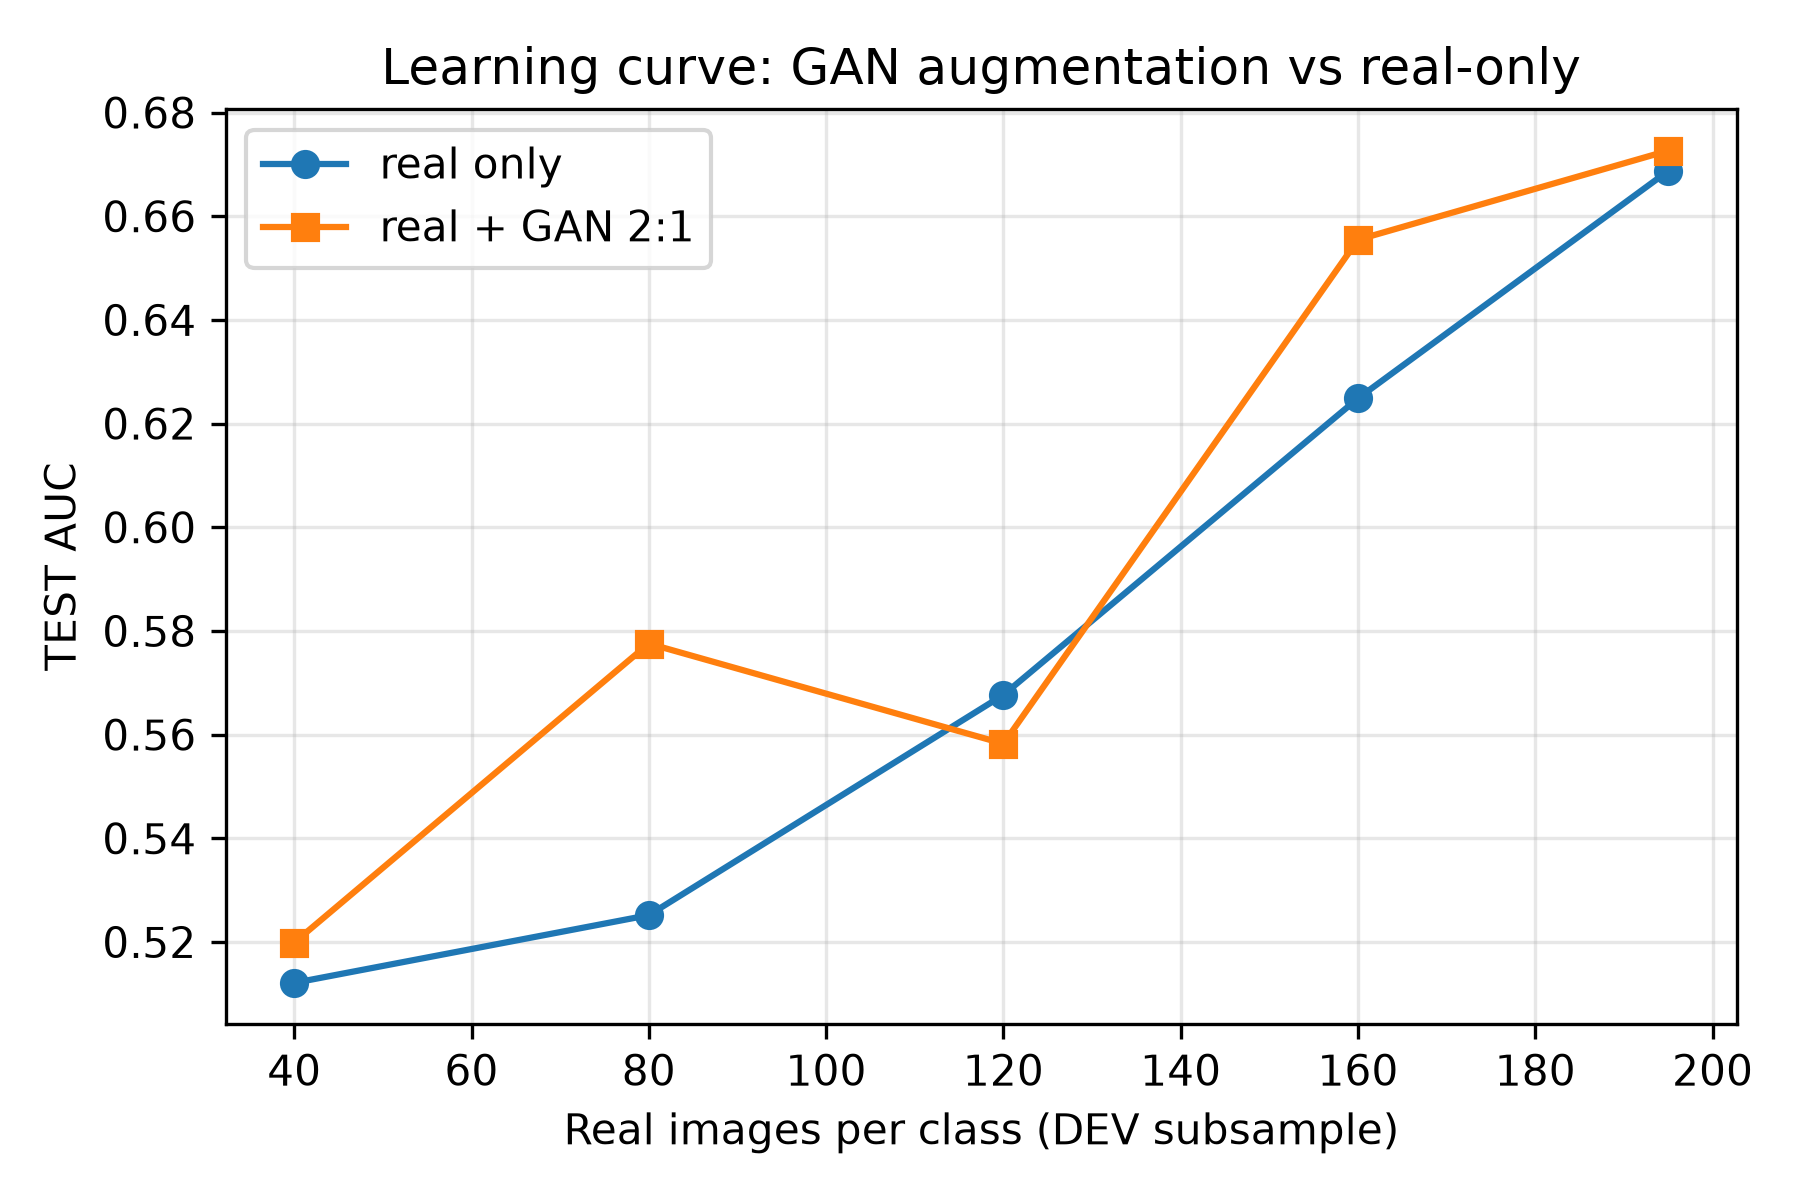
\includegraphics[width=0.6\textwidth]{figures/learning_curve.png}
\caption{Curva de aprendizado: AUC no TEST de treino apenas-real vs aumentado por
GAN (2:1) conforme o conjunto DEV real é subamostrado. A GAN não oferece
benefício consistente ou significativo em nenhum tamanho de dados.}
\label{fig:lc}
\end{figure}

\subsection{Validação Externa}
Para investigar a generalização além do CBIS-DDSM (Revisor 2), o classificador
treinado no CBIS é avaliado \emph{sem qualquer retreinamento} em um conjunto de
dados independente (MIAS; 115 filmes anormais, 63 benignos / 52 malignos,
compatibilizado com a tarefa pela exclusão de filmes normais), usando o mesmo
protocolo com o conjunto externo no lugar do conjunto de TEST travado
(Tabela~\ref{tab:external}). O desfecho coincide com o interno e é novamente
\textbf{negativo}: o modelo mal excede o acaso no MIAS (AUC apenas com dados reais
$0.531$), e a aumentação \emph{não ajuda}---toda proporção aumentada fica no ou
abaixo da linha de base apenas com dados reais ($0.513$--$0.530$), sem diferença
significativa. A grande lacuna de domínio---filme digitalizado versus mamografia
digital de campo total, scanner e população diferentes, e subamostragem agressiva
de $1024\!\to\!128$---significa que o modelo treinado no CBIS não transfere, e a
aumentação sintética não oferece robustez a isso. Isso reforça que o estudo é uma
análise exploratória de viabilidade, não uma evidência de robustez clínica.

\begin{table}[t]
\centering
\caption{Validação externa no MIAS (modelo treinado no CBIS-DDSM completo, sem
retreinamento). Toda proporção fica no ou abaixo do acaso. Regenerada por
\texttt{scripts/06} + \texttt{05}.}
\label{tab:external}
\begin{tabular}{lc}
\toprule
Sintético:Real & AUC (MIAS) \\
\midrule
Apenas reais & 0.531 \\
1:1 & 0.530 \\
2:1 & 0.522 \\
3:1 & 0.521 \\
4:1 & 0.513 \\
\bottomrule
\end{tabular}
\end{table}

% ============================================================================
\section{Discussão}
% ============================================================================
Sob o protocolo com poder estatístico, livre de vazamento e em nível de paciente,
a aumentação sintética não oferece \textbf{nenhum benefício mensurável para
qualquer dos geradores}: a linha de base apenas com dados reais é a configuração
mais forte e nenhuma proporção aumentada é significativamente diferente dela,
sejam as imagens sintéticas provenientes da GAN ou do modelo de difusão, e sejam
avaliadas internamente ou no MIAS. O resultado mais informativo é que o gerador de
\emph{difusão}---que é mais realista (menor FID), mais diverso e apresenta zero
memorização---\emph{ainda assim} não produz nada subsequente. \textbf{A qualidade
do gerador, portanto, não é o gargalo}: elevar a fidelidade da GAN para um modelo
de difusão de estado da arte não move o classificador.

A história do vazamento é \textbf{matizada}. No conjunto de dados completo e com
poder estatístico, mesmo a divisão em \emph{nível de imagem} (vazada), na qual
visões do mesmo paciente podem cruzar treino e teste, dá um resultado
\textbf{nulo} (AUC apenas com dados reais $0.722$; aumentada $0.721$--$0.736$;
todas n.s.). O ganho ``significativo'' espúrio de AUC $0.611\!\to\!0.683$ em
2:1--3:1 (Wilcoxon corrigido por Holm $p_\text{adj}{=}0.047$) aparece
\textbf{apenas} no pequeno subconjunto de $553$ imagens \emph{sob} divisão em
nível de imagem. Em outras palavras, o falso positivo requer \emph{tanto} dados
pequenos \emph{quanto} vazamento: com poder adequado ele não aparece nem mesmo sob
a divisão vazada. Isso torna os ganhos comumente reportados recuperáveis como um
artefato da combinação de amostra-pequena-mais-vazamento, e não dos dados
sintéticos.

A comparação de estratégias de aumento aguça a mensagem prática: a GAN iguala,
mas não supera, o aumento clássico barato ou nem mesmo a ausência de aumento
(Tabela~\ref{tab:augcompare}), de modo que seu considerável custo de treinamento
não compra acurácia; e a análise de poucos dados (Fig.~\ref{fig:lc}) não encontra
nenhum tamanho de dados no qual a GAN ajude de forma confiável, contrariando a
intuição comum de que os dados sintéticos resgatam o regime de poucas amostras.
Não afirmamos que a aumentação sintética \emph{não possa} ajudar a classificação
de mamografias; mostramos que, ao longo de duas famílias de geradores e sob uma
avaliação com poder estatístico e rigorosa, os ganhos comumente reportados não se
reproduzem, e que melhorar a fidelidade do gerador por si só não é suficiente para
produzir um.

% ============================================================================
\section{Limitações}
% ============================================================================
Este estudo reporta um resultado negativo com poder estatístico, não uma
evidência de robustez clínica. (1) O gerador de difusão é construído sobre uma
\textbf{base Stable Diffusion 1.5 pré-treinada em imagens naturais}, de modo que
uma \textbf{lacuna de domínio} separa seu prior da mamografia; adaptar uma base de
difusão pré-treinada em dados \emph{médicos} é uma via natural para trabalhos
futuros, embora nosso achado de que a fidelidade não impulsiona o benefício
subsequente modere a expectativa de que isso mudaria a conclusão. (2) A resolução
de $128\times128$ descarta detalhes diagnósticos finos (margens, textura,
microcalcificações) e restringe a qualidade do gerador. (3) A validação externa
usa um \textbf{único} conjunto de dados adicional (MIAS, filme digitalizado); uma
validação mais ampla multi-institucional/multi-scanner (INbreast, VinDr-Mammo)
permanece como trabalho futuro. (4) Tanto a AUC de linha de base quanto as
aumentadas são moderadas; o modelo não é clinicamente validado, e nenhuma
avaliação prospectiva ou por especialistas foi realizada. (5) Os geradores são
treinados uma única vez em DEV no protocolo reportado; a variante por dobra é
fornecida, mas não executada em escala devido ao custo computacional.

% ============================================================================
\section{Conclusão}
% ============================================================================
Apresentamos um protocolo com poder estatístico, livre de vazamento e em nível de
paciente (TEST travado $n{=}504$) para avaliar a aumentação sintética na
classificação de mamografias de câncer de mama, com uma etapa de seleção
justificada e auditada quanto à memorização, reporte de FID/KID e teste
estatístico completo, e o aplicamos a \emph{duas} famílias de geradores---um
StyleGAN2-ADA e um Stable Diffusion 1.5 ajustado por fine-tuning com LoRA. Sob
este protocolo, \textbf{nenhum dos geradores oferece benefício significativo},
interna ou externamente. Surpreendentemente, o gerador de difusão é mais realista,
mais diverso e livre de memorização, mas ainda assim não produz nada
subsequente---portanto \textbf{a qualidade do gerador não é o gargalo}. Uma
ablação matizada mostra que o resultado positivo reportado sob protocolos mais
fracos requer \emph{tanto} um subconjunto pequeno \emph{quanto} vazamento em nível
de imagem; com poder adequado ele não aparece nem mesmo sob a divisão vazada. A
contribuição é uma demonstração cautelar e reprodutível de que o rigor da
avaliação e o poder estatístico---não a presença ou a fidelidade de dados
sintéticos---impulsionam as melhorias reportadas. Trabalhos futuros: bases de
difusão pré-treinadas em dados médicos; geradores de maior resolução; validação
externa multi-scanner; e o protocolo por dobra em escala.

\subsubsection*{Agradecimentos.} Os autores agradecem ao Departamento de
Computação da Universidade Estadual de Londrina.

\subsubsection*{Disponibilidade de Dados e Código.} O código, as configurações, os
testes e o checkpoint do gerador treinado (Git LFS) são disponibilizados no
repositório do projeto.

\bibliographystyle{splncs04}
\bibliography{references}

\end{document}
